\documentclass{beamer}
\usepackage[utf8]{inputenc}

\usetheme{Madrid}
\usecolortheme{default}
\usepackage{amsmath,amssymb,amsfonts,amsthm}
\usepackage{txfonts}
\usepackage{tkz-euclide}
\usepackage{listings}
\usepackage{adjustbox}
\usepackage{array}
\usepackage{tabularx}
\usepackage{gvv}
\usepackage{lmodern}
\usepackage{circuitikz}
\usepackage{tikz}
\usepackage{graphicx}

\setbeamertemplate{page number in head/foot}[totalframenumber]

\usepackage{tcolorbox}
\tcbuselibrary{minted,breakable,xparse,skins}



\definecolor{bg}{gray}{0.95}
\DeclareTCBListing{mintedbox}{O{}m!O{}}{%
	breakable=true,
	listing engine=minted,
	listing only,
	minted language=#2,
	minted style=default,
	minted options={%
		linenos,
		gobble=0,
		breaklines=true,
		breakafter=,,
		fontsize=\small,
		numbersep=8pt,
		#1},
	boxsep=0pt,
	left skip=0pt,
	right skip=0pt,
	left=25pt,
	right=0pt,
	top=3pt,
	bottom=3pt,
	arc=5pt,
	leftrule=0pt,
	rightrule=0pt,
	bottomrule=2pt,
	toprule=2pt,
	colback=bg,
	colframe=orange!70,
	enhanced,
	overlay={%
		\begin{tcbclipinterior}
			\fill[orange!20!white] (frame.south west) rectangle ([xshift=20pt]frame.north west);
	\end{tcbclipinterior}},
	#3,
}
\lstset{
	language=C,
	basicstyle=\ttfamily\small,
	keywordstyle=\color{blue},
	stringstyle=\color{orange},
	commentstyle=\color{green!60!black},
	numbers=left,
	numberstyle=\tiny\color{gray},
	breaklines=true,
	showstringspaces=false,
}
%------------------------------------------------------------
%This block of code defines the information to appear in the
%Title page
\title %optional
{4.7.44}
%\subtitle{A short story}

\author % (optional)
{RAVULA SHASHANK REDDY - EE25BTECH11047}

 \begin{document}
	
	
	\frame{\titlepage}
	\begin{frame}{Question}
Find the distance of the plane from the origin.
\begin{align*}
\vec{r}^T\myvec{\tfrac{2}{7}\\[4pt]\tfrac{3}{7}\\[4pt]-\tfrac{6}{7}} = 1
\end{align*}

\end{frame}
\begin{frame}{Equation}
Plane Equation
\begin{align*}
    \vec{n}^T\vec{x}=1
\end{align*}
 Distance of a point from a plane
 \begin{align*}
      d &= \frac{|\vec{n}^T \vec{x} - 1|}{\|\vec{n}\|}.
 \end{align*}
\end{frame}

\begin{frame}{Solution}
    Equation of plane
\begin{align}
    \vec{n}^T \vec{x} &= 1,\\
    \vec{n} &= \myvec{\tfrac{2}{7}\\[4pt]\tfrac{3}{7}\\[4pt]-\tfrac{6}{7}}.\\
    d &= \frac{|\vec{n}^T \vec{x}_0 - 1|}{\|\vec{n}\|}.\\
    d &= \frac{|\vec{n}^T \vec{0} - 1|}{\|\vec{n}\|} \\
      &= \frac{|0 - 1|}{\|\vec{n}\|} \\
      &= \frac{1}{\|\vec{n}\|}.\\
      \end{align}
      \end{frame}
      \begin{frame}{Solution}
      \begin{align}
    \|\vec{n}\| &= \sqrt{\vec{n}^T \vec{n}} \\
    &= \sqrt{\left(\tfrac{2}{7}\right)^2 + \left(\tfrac{3}{7}\right)^2 + \left(-\tfrac{6}{7}\right)^2} \\
    &= \sqrt{\tfrac{49}{49}} \\
    &= 1.
\end{align}

Therefore, the required distance is
\begin{align}
    d &= \frac{1}{1} = \boxed{1}.
\end{align}

\end{frame}
\begin{frame}[fragile]
       \frametitle{C Code}
       \begin{lstlisting}
           #include <stdio.h>
#include <math.h>

int main() {
    // Plane normal vector components
    double n[3] = {2.0/7.0, 3.0/7.0, -6.0/7.0};

    // Point (origin)
    double x[3] = {0.0, 0.0, 0.0};

    // Compute n^T x
    double dot = 0.0;
    for (int i = 0; i < 3; i++) {
        dot += n[i] * x[i];
    }
\end{lstlisting}
\end{frame}
\begin{frame}[fragile]
       \frametitle{C Code}
       \begin{lstlisting}

    // Numerator = |n^T x - 1|
    double numerator = fabs(dot - 1.0);

    // Denominator = ||n||
    double norm = sqrt(n[0]*n[0] + n[1]*n[1] + n[2]*n[2]);

    // Distance
    double d = numerator / norm;

    printf("The distance of the plane from the origin is: %.2f\n", d);

    return 0;
}
 \end{lstlisting}
\end{frame}
\begin{frame}[fragile]
       \frametitle{Python Direct Code}
       \begin{lstlisting}
      import numpy as np
import matplotlib.pyplot as plt
from libs.line.funcs   import *  
from libs.triangle.funcs import *   

# --- Plane normal and constant ---
n = np.array([2/7, 3/7, -6/7])
c = 1

# --- Origin ---
origin = np.array([0, 0, 0])

# --- Closest point from origin to plane ---
closest_point = (c / np.dot(n, n)) * n
d = np.linalg.norm(closest_point)

print("Closest point:", closest_point)
print("Distance:", d)
 \end{lstlisting}
\end{frame}
\begin{frame}[fragile]
       \frametitle{Python Direct Code}
       \begin{lstlisting}
# --- Basis vectors lying in the plane ---
u = np.array([n[1], -n[0], 0])
if np.allclose(u, 0):
    u = np.array([0, n[2], -n[1]])
v = np.cross(n, u)

u = u / np.linalg.norm(u) * 2
v = v / np.linalg.norm(v) * 2

# Define four corners of a plane patch (parallelogram)
p1 = closest_point + u + v
p2 = closest_point - u + v
p3 = closest_point - u - v
p4 = closest_point + u - v

# --- Plotting ---
fig = plt.figure(figsize=(8, 6))
ax = fig.add_subplot(111, projection="3d")
 \end{lstlisting}
\end{frame}
\begin{frame}[fragile]
       \frametitle{Python Direct Code}
       \begin{lstlisting}
# Plot plane patch (semi-transparent)
ax.plot_trisurf([p1[0], p2[0], p3[0], p4[0]],
                [p1[1], p2[1], p3[1], p4[1]],
                [p1[2], p2[2], p3[2], p4[2]],
                color="cyan", alpha=0.4)

# Line (Origin → Closest Point)
ax.plot([origin[0], closest_point[0]],
        [origin[1], closest_point[1]],
        [origin[2], closest_point[2]],
        color="black", linestyle="--")

# Origin (red with label)
ax.scatter(*origin, color="red", s=60)
ax.text(*origin, "(0,0,0)", color="red", fontsize=9, weight="bold")
 \end{lstlisting}
\end{frame}
\begin{frame}[fragile]
       \frametitle{Python Direct Code}
       \begin{lstlisting}
# Closest Point (blue with fraction coords as label)
ax.scatter(*closest_point, color="blue", s=60)
ax.text(*closest_point,
        "(2/7, 3/7, -6/7)",
        color="blue", fontsize=9, weight="bold")

# Axes labels
ax.set_xlabel("X-axis")
ax.set_ylabel("Y-axis")
ax.set_zlabel("Z-axis")
ax.set_title("Plane with Closest Point from Origin")

plt.show()
\end{lstlisting}
\end{frame}
\begin{frame}[fragile]
       \frametitle{Python Shared}
       \begin{lstlisting}
import ctypes
import matplotlib.pyplot as plt
from mpl_toolkits.mplot3d import Axes3D

# Define a simple vector class using ctypes
class MyVec(ctypes.Structure):
    _fields_ = [("x", ctypes.c_double),
                ("y", ctypes.c_double),
                ("z", ctypes.c_double)]
    
    def __repr__(self):
        return f"({self.x}, {self.y}, {self.z})"

# Plane normal n and constant d for n^T x = 1
n = MyVec(2/7, 3/7, -6/7)
d = 1
\end{lstlisting}
\end{frame}
\begin{frame}[fragile]
       \frametitle{Python Shared}
       \begin{lstlisting}
# Distance from origin formula: |d| / ||n||
norm_n = (n.x**2 + n.y**2 + n.z**2)**0.5
distance = abs(d) / norm_n
print("Distance of plane from origin:", distance)

# Plotting the plane
fig = plt.figure()
ax = fig.add_subplot(111, projection='3d')

# Create a grid
xx, yy = np.meshgrid(range(-10, 11), range(-10, 11))
# Solve for z using plane equation: n^T x = 1 -> z = (1 - n_x*x - n_y*y)/n_z
zz = (d - n.x*xx - n.y*yy) / n.z
\end{lstlisting}
\end{frame}
\begin{frame}[fragile]
       \frametitle{Python Shared}
       \begin{lstlisting}
# Plot the plane
ax.plot_surface(xx, yy, zz, alpha=0.5, color='cyan')

# Plot the origin and normal vector
ax.scatter(0, 0, 0, color='red', s=100, label='Origin')
ax.quiver(0, 0, 0, n.x, n.y, n.z, length=5, color='blue', label='Normal n')

ax.set_xlabel('X')
ax.set_ylabel('Y')
ax.set_zlabel('Z')
ax.set_title('Plane and its normal vector')
ax.legend()
plt.show()
\end{lstlisting}
\end{frame}
\begin{frame}{Plot}
    \begin{figure}
        \centering
        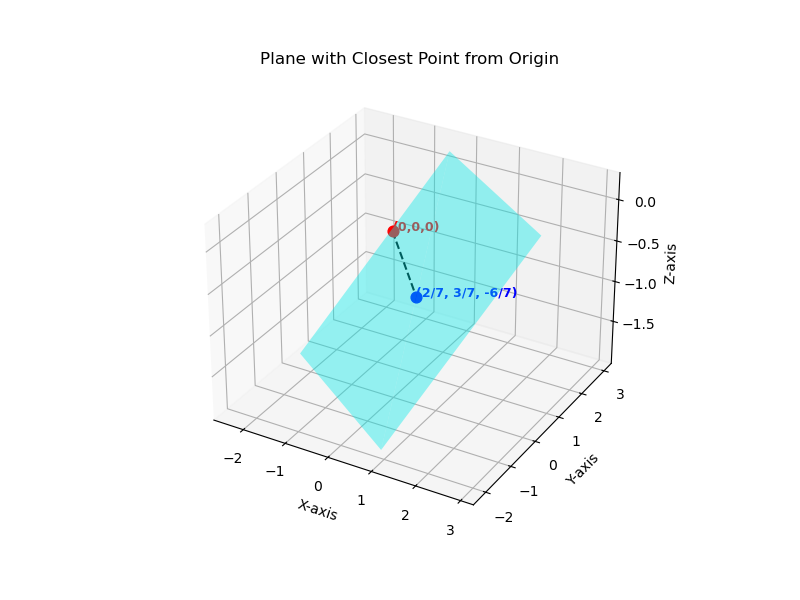
\includegraphics[width=0.75\linewidth]{figs/fig1.png}
        \caption{}
        \label{fig:placeholder}
    \end{figure}
\end{frame}
\end{document}